\chapter{Mesure du temps d'exécution apres 30 fois}
Le tableau suivant représente les temps d'exécution des six algorithmes  30 fois d'itérations sur des nombres ayant des longueurs différentes.
\\
\par
\small
\resizebox{17cm}{!}{
\begin{tabular}{| c | c | c | c | c | c | c | }
    \hline
    Nombre premier &  A1 & A2 & A3 & A4 & A5 & A6   \\
    \hline
 314159    &  0.003033 & 0.001400 & 0.000000  & 0.002200  & 0.000900   & 0.000033  
 \\
    \hline
4480649 &
0.040700 &
0.019367  &
0.000033   &
0.023600s &
0.005822  &
0.000033  \\
    \hline
    50943779 & 0.479900	& 0.231167 &	0.000200	& 0.332567 &	0.011132	& 0.000500  \\
    \hline
    999999937 & 8.502600	& 4.378000	& 0.000633	& 7.151200	& 2.185066 &	0.001267 \\
    \hline
    5915587277 & 49.763900 &	27.214133 &	0.001567 &	25.666167 &	12.863833 &	0.001767  \\
    \hline
    41996139943 & 795.541433 &	186.160400	& 0.003767	& 247.778366	& 92.497733 &	0.004233 \\
    \hline
    100123456789 & 957.670200 &	519.229133	& 0.006333 &	466.633330	& 268.685000 &	0.007533 \\
     \hline
\end{tabular}}
\\ \\
\normalsize
\par
La figure suivante (voir Figure \ref{fig:chart}) représente l'évolution du temps d'exécution selon l'algorithme utilisee.

\begin{figure}[H]
    \centering
        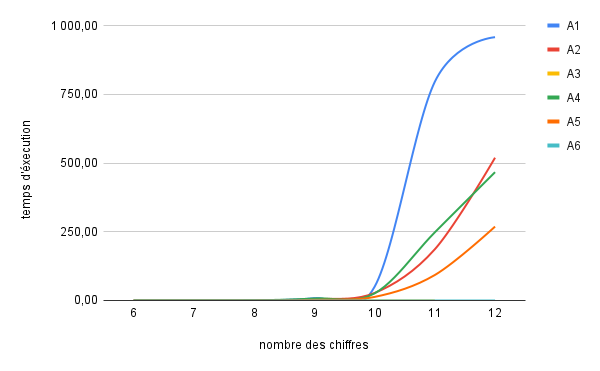
\includegraphics[scale=0.7]{chart2.png}
        \caption{Temps d'exécution des six algorithmes aprés 30 exécutions sur des nombres de longueurs différentes}
    \label{fig:chart}
\end{figure}
\\ 
A partir du graphe ci dessus, on constate qu'il y a une relation de correlation directe entre le nombre de chiffres et le temps d'éxecution moyen (plus que le nombre de chiffres auguemente plus que le temps d'éxecution auguemente)ce qui est le cas pour les algorithmes A1,A2,A4,A5.
\\
Pour le cas des algorithmes A3 et A6, on remarque que le résultat d'exécution tend vers 0 malgré l'augmentation du nombre de chiffres. 
